\section{Installation}
To use it you need the following to be installed on your system
\begin{itemize}
    \item \codet{Python 2.7.x}
    \item Packages for \codet{Python 2.7.x}:
            \begin{itemize}
                \item \codet{Tkinter}
                \item \codet{ttk}
                \item \codet{tkFont}
                \item \codet{tkFileDialog}
            \end{itemize}
\end{itemize} 
Most probably all of the above packages are already installed provided \codet{Python 2.7}
is installed on your system.

Provided the above dependencies are installed you are ready to use it. Change to
\codet{gui} directory. There you will find the file named \codet{caenccf}. You may need
to make it executable. On Ubuntu the following command does the work:
\begin{lstlisting}
> chmod +x caenccf
\end{lstlisting}
Now just run it
\begin{lstlisting}
> ./caenccf
\end{lstlisting}
If everything is OK you should see the following window on your screen:
\begin{figure}[H]
    \centering
    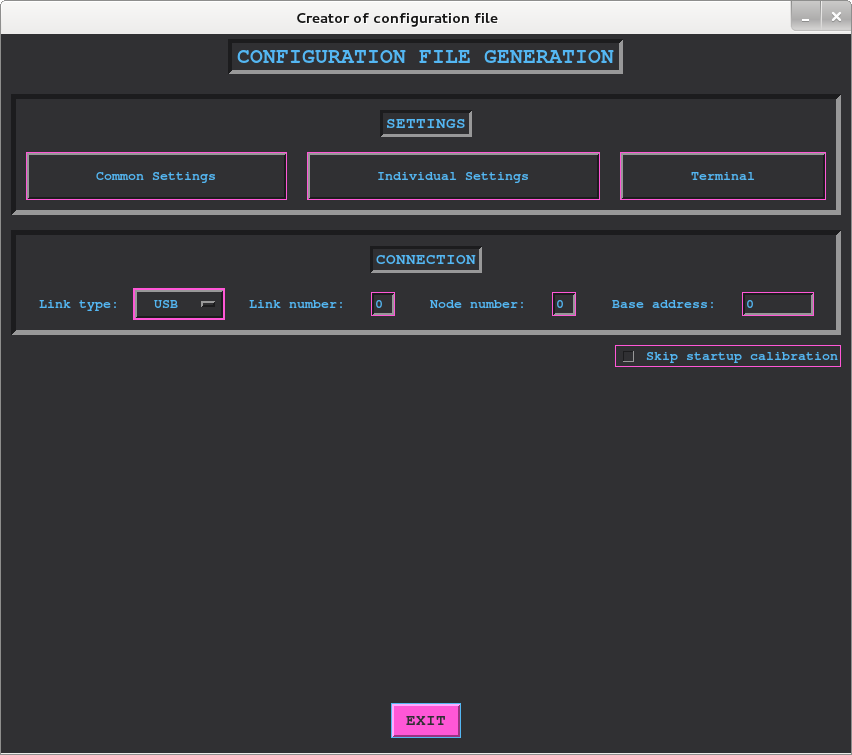
\includegraphics[width=0.8\textwidth]{../pictures/documentation/gui/start_page.png}
    \caption{GUI starting page}
    \label{fig:gui_stpg}
\end{figure}

It is very useful to be able to run it from everywhere on your system. In order to reach
this you need to place the executable in your \codet{bin} directory:
\begin{lstlisting}
> cp caenccf /usr/bin/
\end{lstlisting}
Also you need to extend the \codet{PYTHONPATH} environment variable in order \codet{Python}
to see necessary modules. On Ubuntu add the following line in your \codet{.bashrc} file:
\begin{lstlisting}
export PYTHONPATH=$PYTHONPATH:/path/to/<package_dir>/gui
\end{lstlisting}
After that you should be able to run the GUI from anywhere on your system. 
